\section{Analysis of the Experiment}
\label{sec:Auswertung}



\subsection{LED to Laserdiode}
\label{sec:LED_Laser}
First a threshold current of
\begin{align}
I_{\mathrm{threshold}} = \SI{}{\ampere}
\end{align}
is measured.
Futhermore in Figure \ref{fig:threshold} the two
pictures from the Kamera focusing on the card are showen.
With the different that on one picture the current of the diode is below threshold \ref{fig:LED} and
on the other above threshold \ref{fig:LASER}.
\begin{figure}
  \centering
  \begin{subfigure}{0.45\textwidth}
    \centering
    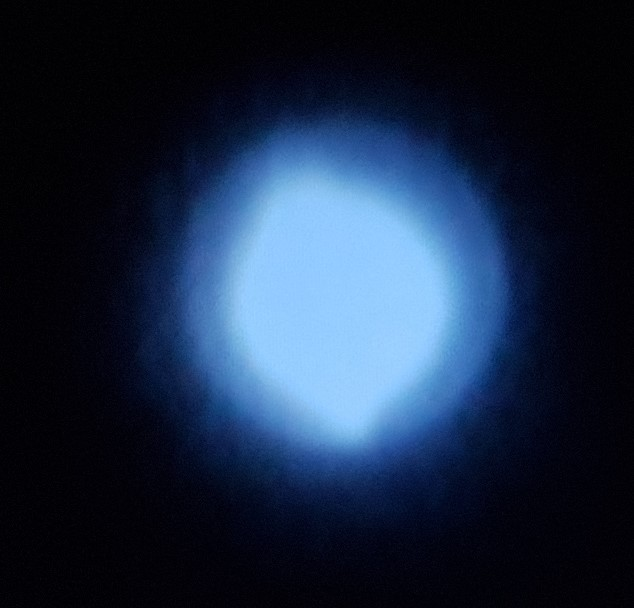
\includegraphics[height = 5cm]{figures/bevore_threshole.jpg}
    \caption{LED}
    \label{fig:LED}
  \end{subfigure}
  \begin{subfigure}{0.45\textwidth}
    \centering
    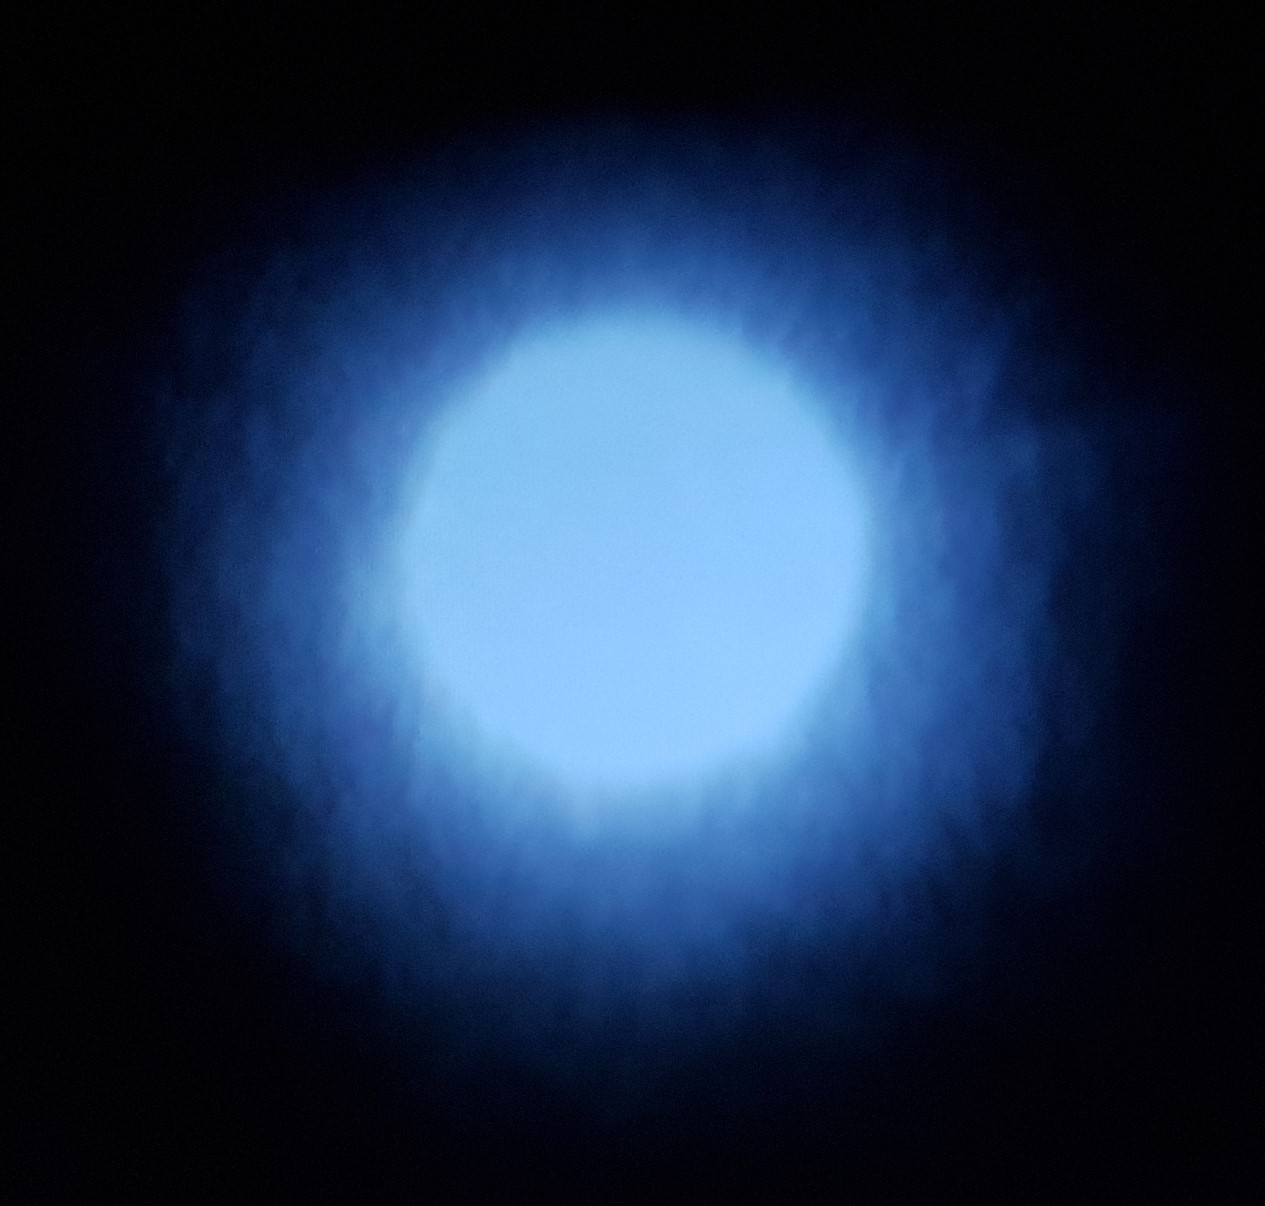
\includegraphics[height = 5cm]{figures/after_threshole.jpg}
    \caption{LASER}
    \label{fig:LASER}
  \end{subfigure}
\caption{The light below \ref{fig:LED} and above \ref{fig:LASER} the current threshold.}
\label{fig:threshold}
\end{figure}
The intensity change of the diode beam is clearly recognisable
between the lower intensity LED radiation \ref{fig:LED}
and the higher LASER radiation\ref{fig:LASER}.
% so the theory of a threshold current can be confirmed.

It follows the results for the setup \ref{fig:setup2}.
First with the Rubidum absorption cell loceated in the laser beam
and the current adjusted so Rubidum fluorescence is observed, the picture of the
Kamera, which is targeted at the
Rubidum absorption cell, is
displayed in the figure \ref{fig:Floures}.

\begin{figure}
  \centering
  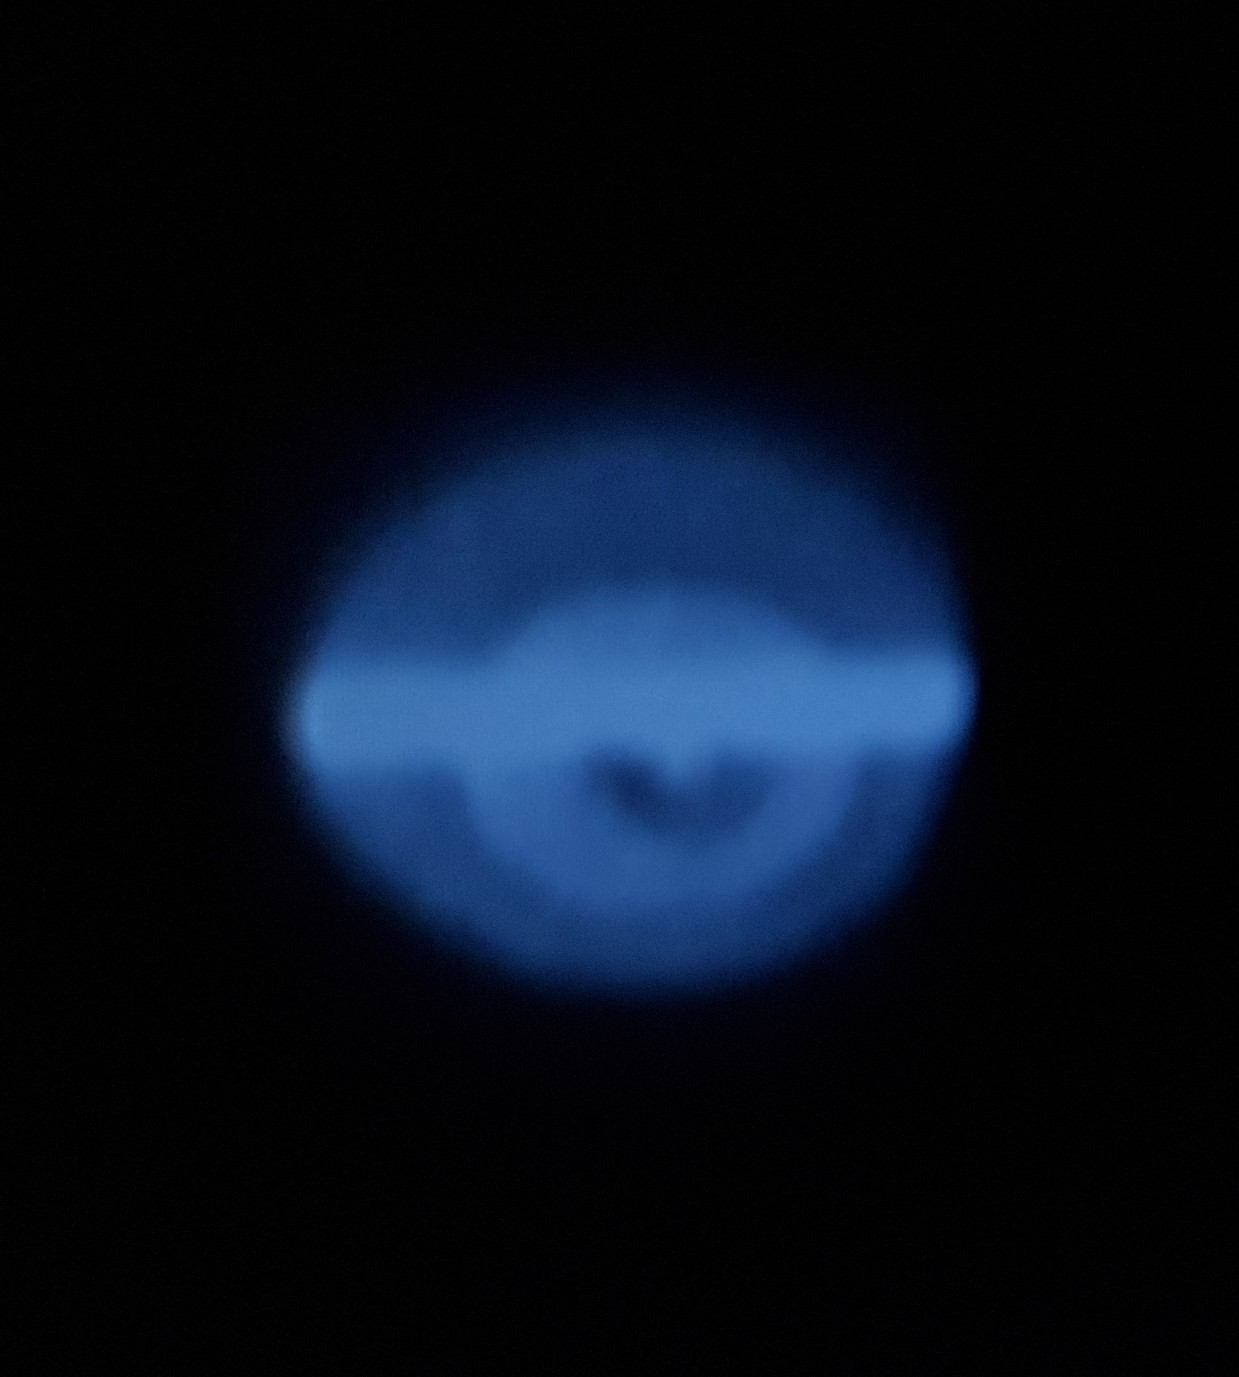
\includegraphics[width = 0.5\textwidth]{figures/Rb_leuchten.jpg}
  \caption{Rubidum }
  \label{fig:Floures}
\end{figure}

Rubidum flourescence is only observe in the Laser beam therfore
the brighter horizontal line
in figure \ref{fig:Floures}
is the track of the laser beam
goes through the Rubidium cell and stimulates the Rubidum atoms.

Now with the active ramp generator moving the grating with the piezo stack,
the signal from the photodiode behind the rubidum cell
is displayed with a
oscilloscope and shown in figure \ref{fig:ramp}.
Also the signal of the ramp generator is shown at the same
figure.

\begin{figure}
  \centering
  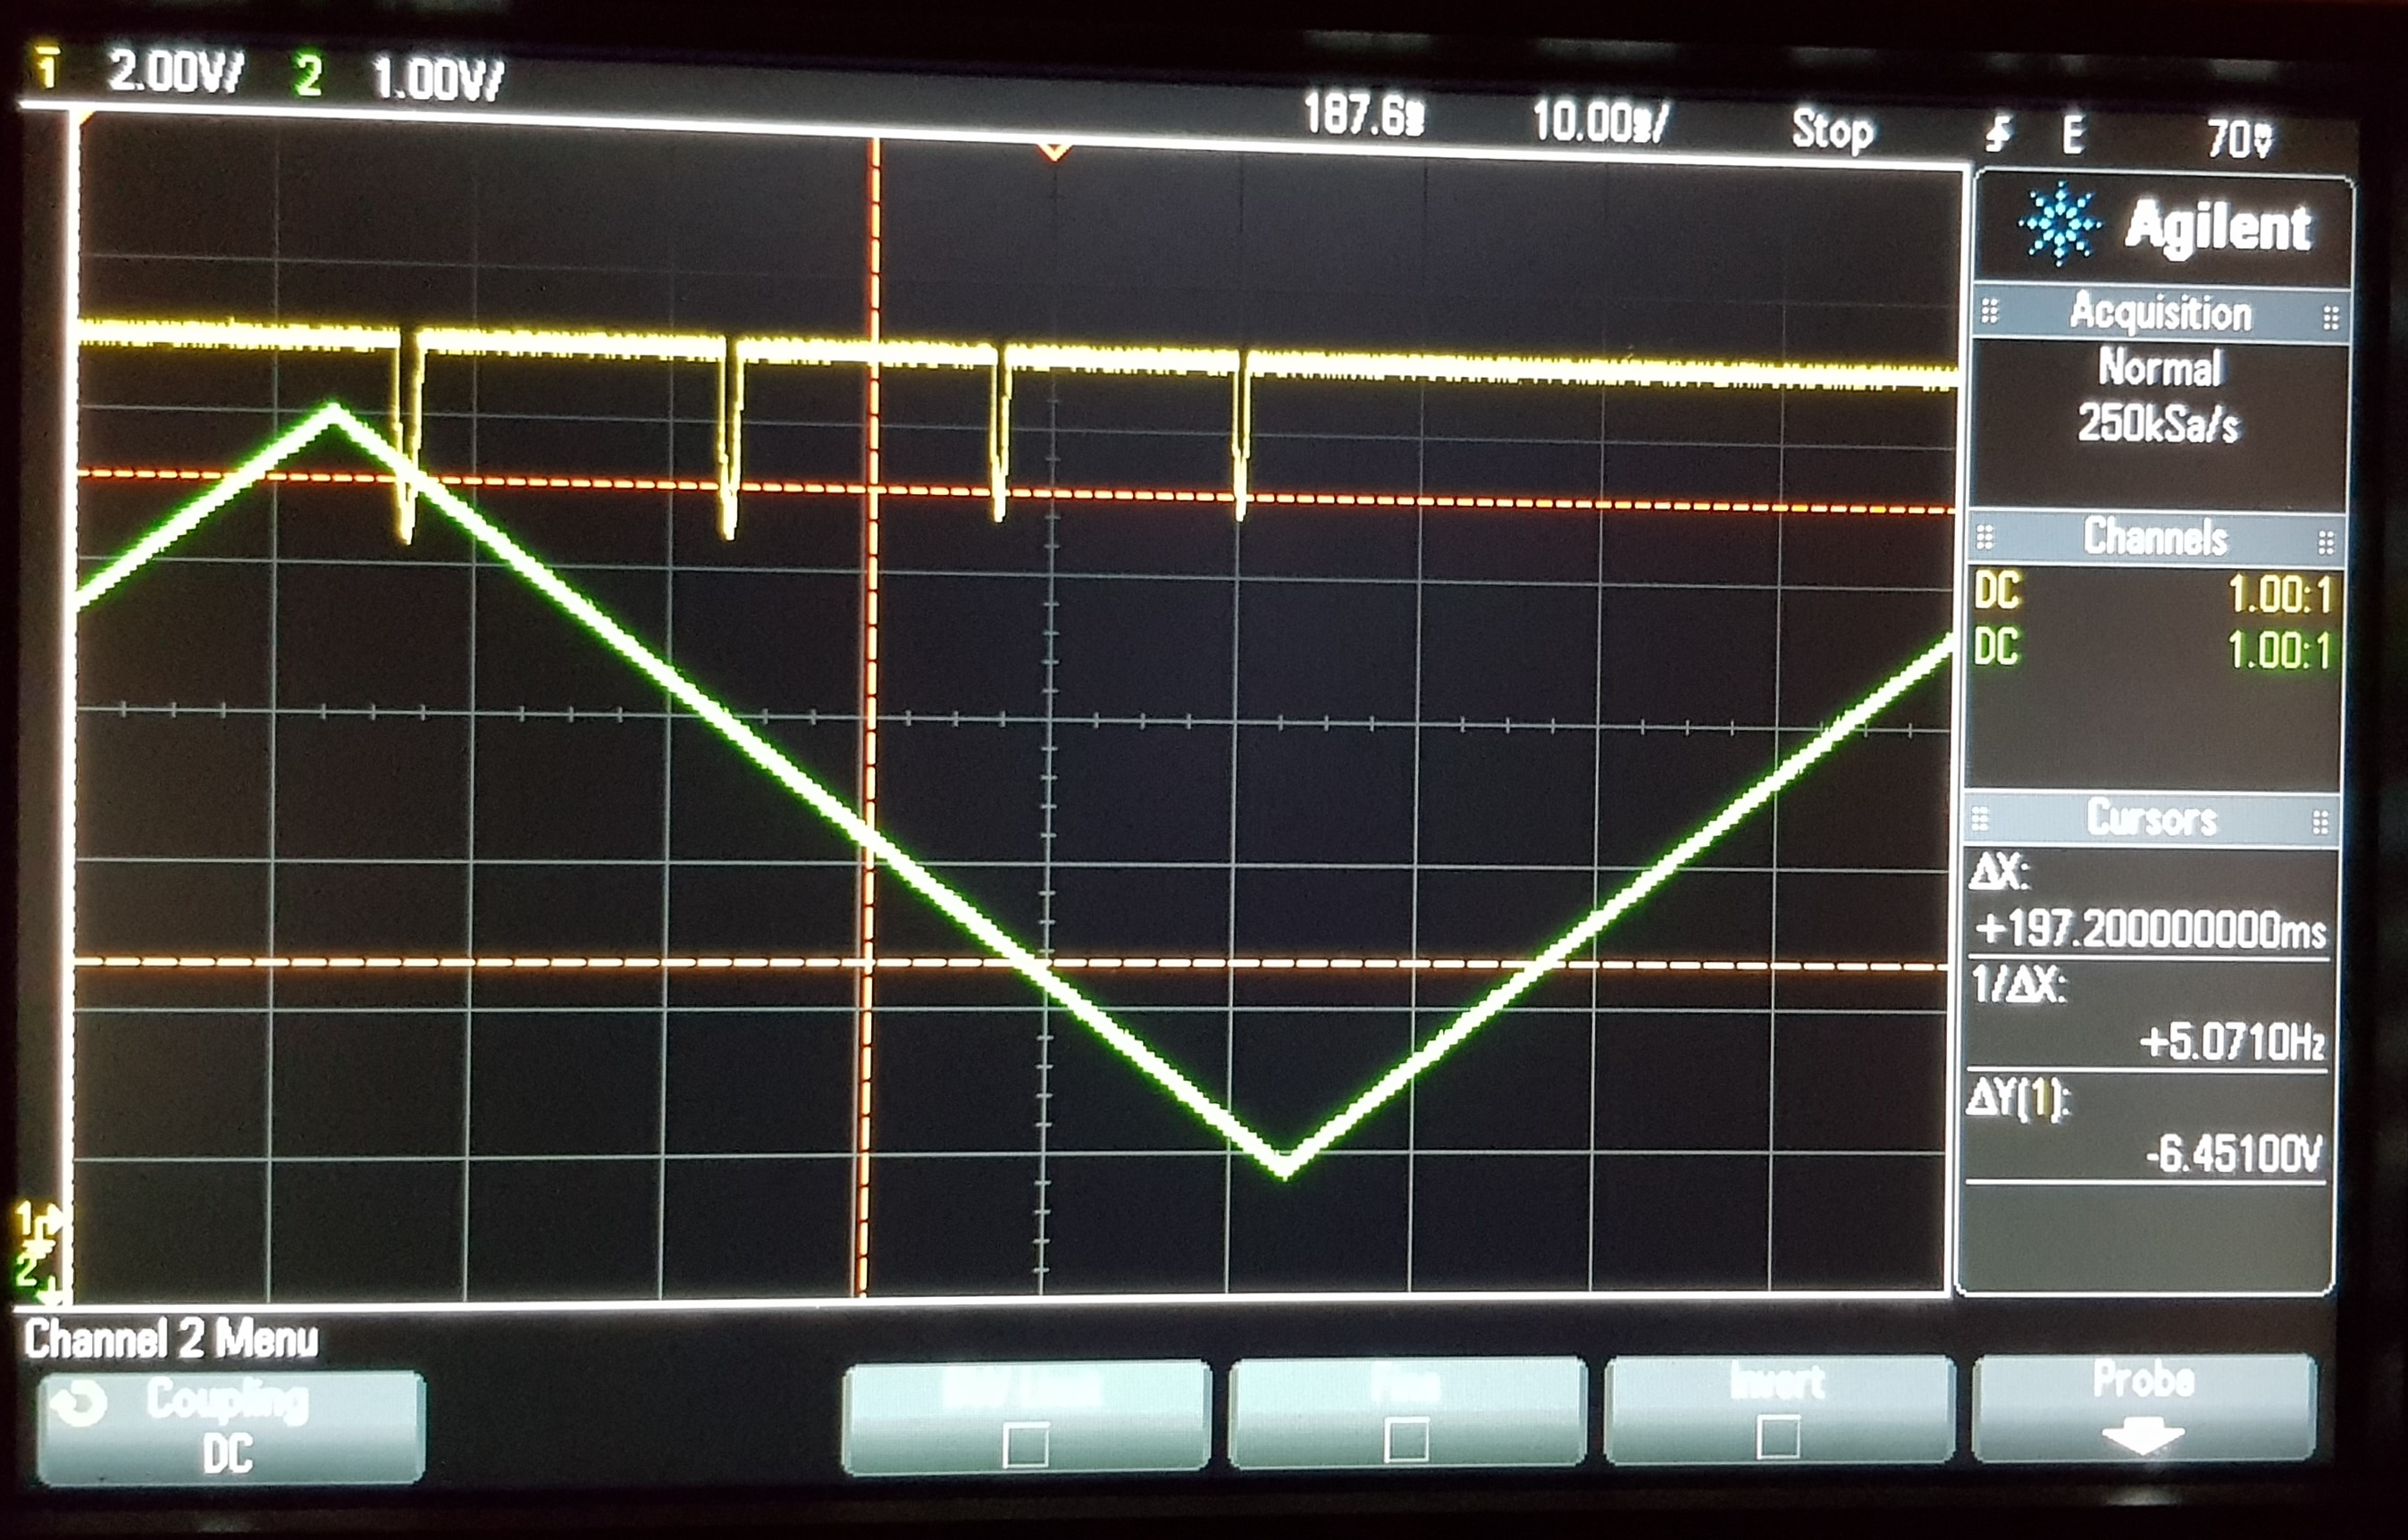
\includegraphics[width = 0.7\textwidth]{figures/Ramp.jpg}
  \caption{Signal from the photodiode and the ramp generator.}
  \label{fig:ramp}
\end{figure}




\subsection{Rubidum absoptionspectrum}
\label{sec:ru_absoption}
